\documentclass[12pt,letterpaper]{exam}
%\usepackage{color}
\usepackage[usenames,dvipsnames,svgnames,table]{xcolor}
\usepackage[margin=0.9in]{geometry}
\renewcommand{\familydefault}{\sfdefault}
\usepackage{multicol}
\pagestyle{head}
\definecolor{c02}{HTML}{FFBBBB}
\definecolor{c03}{HTML}{FFDDDD}
\header{AM 108 Problem Set 03}{}{{\colorbox{c02}{\makebox[3.0cm][l]{Due Fri Feb 17}}}\\ at noon p.\thepage}
\runningheadrule
\headrule
\usepackage{diagbox}
\usepackage{graphicx} % more modern
%\usepackage{subfigure} 
\usepackage{amsmath} 
\usepackage{amssymb} 
%\usepackage{gensymb} 
%\usepackage{natbib}
\usepackage{hyperref}
%\usepackage{enumitem}
%\setlength{\parindent}{0pt}
%\usepackage{setspace}
%\pagestyle{empty}  
%\newcommand{\Sc}[0]{
%{\color{BlueViolet}\S}
%}
\usepackage{tcolorbox}
\usepackage[framed,numbered,autolinebreaks,useliterate]{mcode}

% \renewcommand{\labelenumii}{\theenumii}
% \renewcommand{\theenumii}{\theenumi-\arabic{enumii}.}

\newif\ifprintselans
\printselanstrue
%\printselansfalse
\newenvironment{selans}
{\ifprintselans
   \printanswers
   \renewcommand{\solutiontitle}{\noindent\textbf{Answer:}\par\noindent}
 \fi
}
{}

\newif\ifprintselsol
%\printselsoltrue
\printselsolfalse
\newenvironment{selsol}
{\ifprintselsol
   \printanswers
   \renewcommand{\solutiontitle}{\noindent\textbf{Solution:}\par\noindent}
 \fi
}
{}


\begin{document}
 \pdfpageheight 11in 
  \pdfpagewidth 8.5in

\noindent\textbf{Problem Set Instructions:}  
\begin{itemize}
\itemsep0pt
\item In your first attempt of the problem set problems, you are encouraged to treat the problem set as an open-notes quiz.  Work on it without consulting classmates, Ed, course staff, other people, other internet resources, or any solutions or answers.  Work on each problem, completing as much as you are able to, and making a note in your work whenever you become stuck or confused.
\item After your initial individual attempt, collaboration is encouraged (see guidelines below) as you continue to work on the problems.  You'll submit a pdf of this work as part of your problem set submission on Gradescope (and will also submit it on Canvas).
\item Submit the pdf of your problem set work with the problems written up in order (computational work should be included: it can be at the end of the pdf) on Canvas and access the solutions.
\item Complete the reflection questions below, and submit that reflection work, along with your problem set pdf, on Gradescope.
\end{itemize}
  
\noindent\textbf{Submission Instructions:}  
\begin{itemize}
\item Following the instructions above, upload a pdf of your work to Canvas.  Upload your reflection answers and the pdf to Gradescope.
\item If you would like to use mathematical software other than Mathematica, that's fine. 
\end{itemize}

\noindent\textbf{Late Work Policy:}
\begin{itemize}
\itemsep0pt
\item Problem sets are accepted up to eight hours late with no penalty (8pm Friday). 
\item Three 36 hour late days are available to every student (three extensions to 8pm on Saturday).  These late days are expected to be used for unexpected illness or other conflicts.
\item Additional late days are not typically 
available.
\item Problem sets are not accepted beyond the late deadline.
\end{itemize}

\noindent\textbf{Collaborating on Problem Sets:}  

\noindent Collaborating with classmates in planning and designing solutions to homework problems is encouraged.  Collaboration, cooperation, and consultation can all be productive.  Work with others to: 
\begin{multicols}{2}
\begin{itemize}
\itemsep-0.2em
    \item discuss the problem
    \item brainstorm
    \item walk through possible strategies
    \item outline solution methods
\end{itemize}   
\end{multicols}

\noindent For homework, you may consult or use:
\begin{multicols}{2}
\begin{itemize}
\itemsep-0.2em
    \item Course text (including answers in back)
    \item Your notes (taken during class)
    \item Class notes of other students
    \item Course handouts
    \item Canvas posts/Ed posts
    \item Computational tools such as Python, Mathematica, or Desmos
    \item Calculators
    \item Other books
    \item the Internet
\end{itemize}
\end{multicols}

\noindent You may:
\begin{itemize}
    \item Look at communal work while writing up your own solution
\end{itemize}

\noindent You may \textbf{not}:
\begin{itemize}
\itemsep-0.2em
    \item Look at the individual work of others while writing up your own solutions
    \item Post about problems online
\end{itemize}


\noindent Do \textbf{not} consult the following resources until after you think you have solved a problem, have fully written up your answer, and have submitted a pdf of your work to Canvas.
%\begin{multicols}{2}
\begin{itemize}
\itemsep-0.2em
    \item The text solution manual
    \item The posted solutions
    \item Other solutions (from previous years, from sites like Chegg or Math Stackexchange, etc)
\end{itemize}
%\end{multicols}


%\eject


% \begin{enumerate}
% \item Reflection questions

\section*{Reflection questions}
Submit these on Gradescope.
\begin{enumerate}
\item \begin{enumerate}
    \itemsep0pt
    \item When you worked on the problems individually, how did each problem go?
    \item Where did you get stuck or confused?  For any subpart where you were stuck or confused be specific.  \emph{For example 'I tried to use the hint for 3b, but I couldn't find a way to relate $r$ and $x$'.}
    \item What additional progress were you able to make when you consulted other people or additional resources?
    \item For each part of each problem, how did your work compare with the posted solution?  Identify similarities and differences.
\end{enumerate}  
\item For any problems you were not able to complete, what made them difficult to complete?  What did you learn from the posted solution?
\item What aspects of the course challenged you this week?  What did you do to address those challenges?  What topics/ideas/procedures do you not yet understand?
\item What did you understand the best this week?  What, if anything, do you understand better this week than you did in the past?
\item List the people that you worked with or consulted on the problem set problems.  This might include other students in the course, course instructors, or people who have previously taken the course.
\item Below, indicate how much of your time for this class has been doing the following activities:
	\begin{enumerate}
	\item Working on problem set problems or other practice problems alone
	\item Reviewing course materials, including problem set solutions, alone
	\item Working on problem sets, reviewing notes, or discussing course topics with your classmates
	\item Working through supplementary materials
	\item Going to office hours
	\item Other (please specify)
	\end{enumerate}

\end{enumerate}


\section*{Problems}


\begin{questions}
\question (variation on 3.7.7) We will work on a non-dimensionalized version of the problem from the text.  Consider a protein that activates its own transcription in a positive feedback loop, while its promotor has a certain level of basal expression:
\[\dot{p} = \alpha + \frac{\beta p^n}{K^n+p^n} - \delta p.\]

Here $\alpha$ is the basal transcription rate, $\beta$ is the maximal transcription rate, $K$ is the activation coefficient, and $\delta$ is the decay rate of the protein.  To ease the analysis, assume that $n$ is large ($n\gg 1$).
%\begin{parts}
%\item Explain the setup for the problem in your own words. Include explanations for the following terms: \emph{positive feedback}, \emph{protein transcription},  \emph{promotor}, \emph{basal transcription rate}.  Cite your sources.

Note:  The process of both transcription + translation is probably what is meant by \emph{protein transcription} in this problem.
%\end{parts}

The system can be put in the dimensionless form \[\frac{dx}{d\tau} = s - r x + \frac{x^n}{1+x^n}\] where $r>0$ and $s\geq 0$ are dimensionless groups.  For $n=2$ this equation is identical to the model gene activation on PSet02.

\begin{parts}
%\stepcounter{partno}
\begin{solution}
\end{solution}
\item   For this problem, we assume $n$ is large ($n\gg 1$).  Sketch the graph of the nonlinear function $g(x) = x^n/(1+x^n)$ for a value of $n$ that is very large.  What simple shape does it approach as $n\rightarrow \infty$?
\begin{solution}
\end{solution}
\item The right side of the equation for $\dot{x}$ can be written as $g(x) - h(x)$ where $h(x) = rx - s$.  

Use this decomposition to plot a phase portrait for the system for the following three cases: (i) $r-s>1$ (i.e. $\delta K - \alpha >\beta$ ), (ii) $r-s = 1/2$ (i.e. $\delta K - \alpha = \beta/2$), and (iii) $r-s<0$ (i.e. $\delta K - \alpha < 0$).  

Work with the nondimensional equations for this.  On your phase portrait, label the location of each fixed point (this may need to be in terms of $r$ and $s$).  Also label $x =0$ and $x=1$ on the phase portrait (and make sure your fixed points are drawn in the correct regions of the $x$-axis relative to $0$ and $1$).
\end{parts}

From here on, assume $r > 1$ (i.e. $\delta K > \beta$)

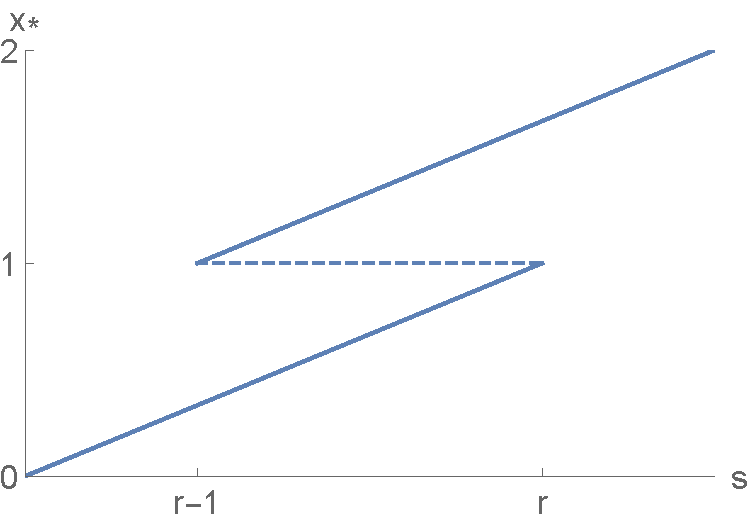
\includegraphics[width=3in]{img/HW03_377_p3.pdf}

\begin{parts}
\setcounter{partno}{2}

\item  A bifurcation diagram for this system is shown above (drawn for $n\rightarrow\infty$).  Bifurcations occur at $s = r-1$ and $s = r$.  
\begin{itemize}
    \item What type of bifurcation is each one?
    \item Explain how your phase portraits relate to this diagram.
\end{itemize}
 
\begin{solution}
\end{solution}
\item Discuss how the level of protein behaves if $\alpha$ is very slowly increased from $s=0$ so $s>r$, and then very slowly decreased back to $s = 0$ (i.e. from $\alpha = 0$ to $\alpha>\delta K$, and then back to $\alpha = 0$).

The term ``hysteresis'' refers to when the current state of the system depends on the history of the state of the system (i.e. knowing the parameters alone is not enough to know the state of the system).  Is there hysteresis in this system?  How did you decide?
\begin{solution}
\end{solution}
\end{parts}


\question Do 4.5.1abc

See the text for this question.  As you work on the question, follow the analysis in Section 4.5: this problem has you do a similar analysis with a different response function.

For \textbf{part d}: 
\begin{itemize}
    \item Set up the integral for $T_{\text{drift}}$ for the function $f$ given in the problem.
    \item Explain what $T_{\text{drift}}$ represents.
    \item What do you expect to happen to $T_{\text{drift}}$ as $\mu$ approaches $\pi/2$ from above?
\end{itemize}
  

% Read section 4.4 to understand the setup of the problem.  We are taking the system described in section 4.4 and adding a spring.  Think of the pendulum as moving through molasses or another thick fluid, where there is so much friction that its motion does not have inertia; instead, if the force on the pendulum stops it will immediately stop moving.  

% For the spring, treat its force as increasing with $\theta$, even if $\theta$ increases past $2pi$. This is different than the angular systems we have encountered before.  Here, the actual angle matters (so for part a you'll explain why this is \textbf{not} well-defined on a circle). 



Show your work for each part. 

\item (inspired by 5.1.2, 5.1.10, and 5.1.11) Consider the system
\[\dot x=-x+y,\quad \dot y=x-ay\] 
	\begin{parts}
	\item Find the trace $\tau$ and the determinant $\Delta$ as a function of $a$.
 \end{parts}
 
 The eigenvalues are $\lambda_\pm=\dfrac{\tau\pm\sqrt{\tau^2-4\Delta}}{2}$.  
 
 The corresponding eigenvectors are
	\[\underline{v}_\pm=\left[\begin{array}{c}
	\Delta\pm\sqrt{\tau^2-4\Delta}\\
	2
	\end{array}\right] = \left[\begin{array}{c}
	a-1\pm\sqrt{a^2-2a+5}\\
	2
	\end{array}\right]\].  The two eigenvectors are orthogonal.
 \begin{parts}
     \setcounter{partno}{1}



 \item For $a = -2, 1, 2$, find the eigenvalues and eigenvectors of the system.  Use Mathematica/Python for this (or work by hand).

%In the $xy$-plane, draw your eigenvectors and try to sketch phase portraits for these three cases.  You should have the correct direction of motion along the eigendirections.

 Generate phase portraits in Mathematica/Python and add lines to your plots along the eigendirections.

%\item What happens to the eigenvectors and phase portraits as $a\to\pm\infty$?

	\item There is a critical $a_c$ (to be determined by you).   Show that for $a<a_c$ the origin is a saddle point and for $a>a_c$ the origin is a stable node. 

 \item (Optional: time permitting) At $a=a_c$ the origin is not an attractor, but it has a property called Liapunov stability, where trajectories that start sufficiently close to the origin stay near it for all time.  (See the end of \S 5.1 in the text).

Let $(x(t),y(t))$ be a trajectory in this system.  Consider the distance to the origin at time $t$, $d(t) = \sqrt{(x(t))^2 + (y(t))^2}$.  Show that $(d(t))^2 = (x(t))^2 + (y(t))^2$ does not increase in time.  To do this, use the chain rule to compute $\frac{d}{dt} (d(t))^2$ and argue that it is always non-positive.

\emph{One approach: 1. Find $\frac{d}{dt} d^2(t)$ in terms of $x, \dot x, y, \dot y$.  2. Use $\dot x = y - x$ and $\dot y = x-ay$ to eliminate the time derivatives from your expression. 3. Rewrite your expression in terms of a square, and argue that $d^2$ (and thus $d$) is never increasing.}
 
\end{parts}
\item (Sketching phase portraits for systems with complex eigenvalues) 

When a system's eigenvalues $\lambda_1$ and $\lambda_2$ are real, the eigenvectors give the straight line solutions into or out of the origin.  When $\lambda_1$ and $\lambda_2$ are complex, the eigenvectors don't provide the same information for sketching the phase portraits.

For $\lambda_\pm=\pm ib$, the origin is a center.  Solutions form concentric ellipses.  On an elliptical trajectory, at the semimajor and semiminor axes, a vector tangent to the trajectory is perpendicular to the axis.

 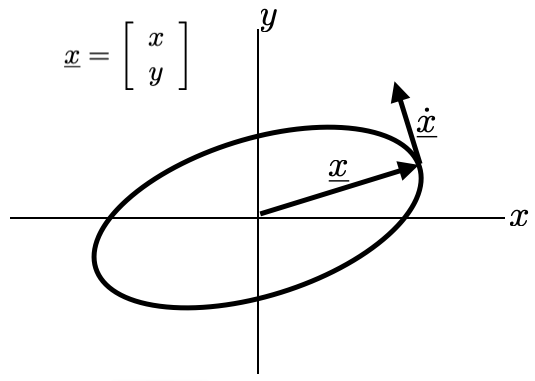
\includegraphics[scale=0.5]{img/PSet03_ellipse.png}
 
   To find these axes we solve the matrix equation 
	\[\underline{x}\cdot \dot{\underline{x}}=0\Rightarrow \underline{x}\cdot A\underline{x}=0\]
	for the vector $\underline{x}$.  Since there are two axes, one of them must have the first coordinate be nonzero, so we can set $\underline{x}=\left[\begin{array}{c}1\\t\end{array}\right]$ and solve for $t$.

	\begin{parts}
	\item 
 
 For the system
	\[\dot x=(-9x+15y)/4\quad \dot y=(-15x+9y)/4\]
	find the eigenvalues and eigenvectors.  
 
 Show that the semimajor and semiminor axes of the solutions lie along the directions
	\[v=\left[\begin{array}{c}
	1\\
	1
	\end{array}\right]
	\quad
	u=\left[\begin{array}{c}
	1\\
	-1
	\end{array}\right].\]
	Note that these directions do not correspond to the real or imaginary parts of the eigenvectors.
	\item Use Python/Mathematica to plot the phase portrait along with the directions of the semimajor and semiminor axes.
	% \item For $\lambda_\pm=a\pm ib$, the same principle as with centers applies.  We can find the $\underline{x}$ so that
	% \[\underline{x}\cdot A\underline{x}=0\]
	% rather than use the eigenvectors. For the system
	% \[\dot x=y\quad \dot y=-4x-2y\]
	% find the eigenvalues and eigenvectors.  Then find the directions $\underline{v}$ and $\underline{u}$ that correspond to the tangent vectors of the solutions being perpendicular to the vector spaces $\text{span}\{\underline{v}\}$ and $\text{span}\{\underline{u}\}$.
	% \item Use Python/Mathematica to plot the phase portrait along with two lines corresponding to the vector spaces you found.
	\end{parts}






 

 \end{questions}




\end{document}
